\documentclass{beamer}

\usepackage[utf8]{inputenc}
\usepackage{graphicx}
\usepackage{amsmath}
\usepackage{amssymb}
\usepackage{minted}
\usepackage{algpseudocode,algorithm,algorithmicx}
\usepackage{tikz}
\usetikzlibrary{shapes,arrows}
\usetikzlibrary{positioning}
\usepackage{bussproofs}
\usepackage[backend=biber]{biblatex}
\addbibresource{citations.bib}

\title{Formalizing Graph Theory in Type Theory}
\subtitle{with progress towards a formalization of Wigderson's algorithm}
\author{Siraphob Phipathananunth}
\date{\today}
\institute{Vanderbilt University}

\begin{document}

\frame{\titlepage}

\begin{frame}
\frametitle{Outline}
\tableofcontents
\end{frame}

\begin{frame}
\frametitle{Introduction and motivation}
\begin{itemize}
\item Formalist approach to mathematics since Euclid
\item Modern analogue: mechanized proofs
\item Examples: four-color theorem, Kepler conjecture, time invariance thesis for weak call-by-value $\lambda$-calculus
\item Motivation: proving correctness Wigderson's algorithm in Coq
\end{itemize}
\end{frame}

\begin{frame}

\includegraphics[width=\textwidth]{./images/gonthier.png}
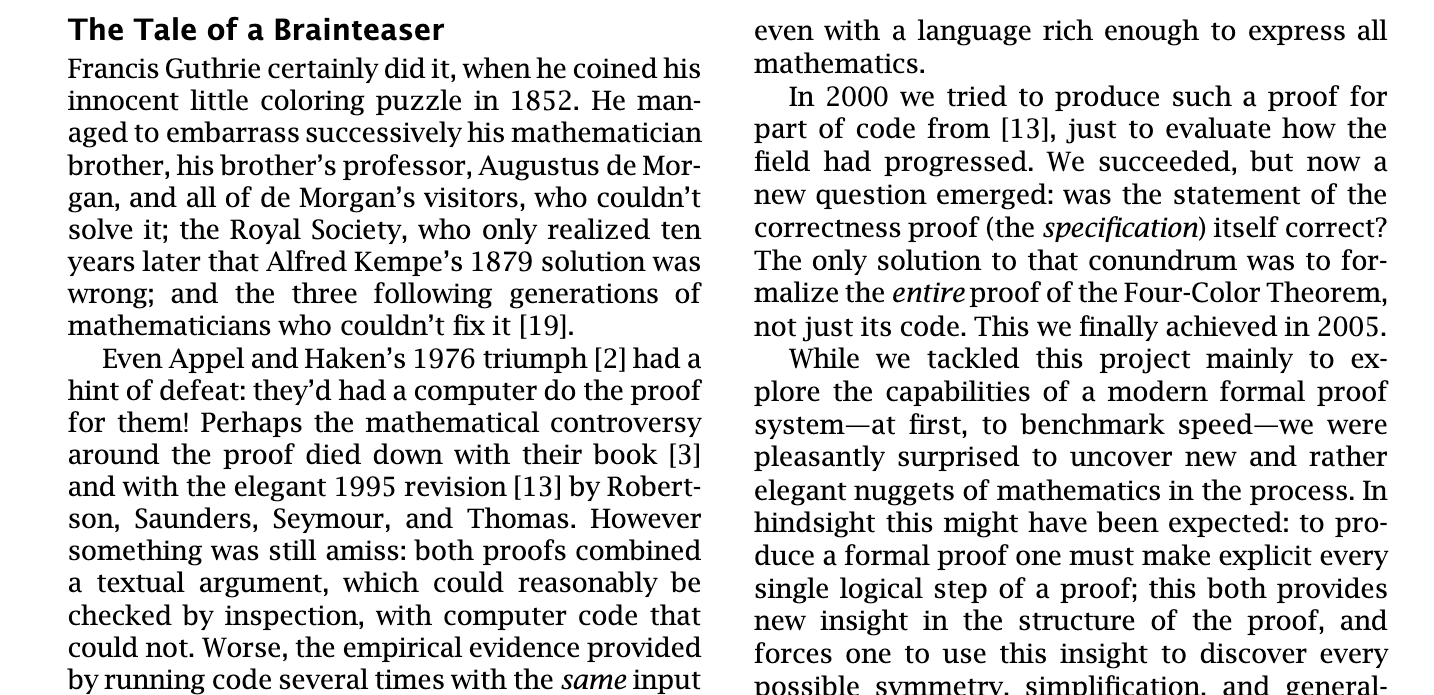
\includegraphics[width=\textwidth]{./images/gonthier-text.png}
\end{frame}

\section{Background}
\begin{frame}
\frametitle{Background}
\begin{itemize}
\item Interdisciplinary work involving logic, type theory, graph theory, and computer science
\item Use of Coq proof assistant
\item Applicability and simplicity of graph theory
\item Computability of graph algorithms
\end{itemize}
\end{frame}

\subsection{Dependent type theory}
\begin{frame}
\frametitle{Dependent type theory}
\begin{itemize}
\item Type theory: alternative to set theory for the foundation of mathematics
\item Dependent types: types that depend on values
\item Progression of type theories: STLC, System F, Calculus of Constructions
\end{itemize}
\end{frame}

\begin{frame}
\frametitle{STLC: Simply Typed Lambda Calculus}
\begin{prooftree}
\AxiomC{$x : A \in \Gamma$}
\RightLabel{(var)}
\UnaryInfC{$\Gamma \vdash x : A$}
\end{prooftree}

\begin{prooftree}
\AxiomC{$\Gamma, x : A \vdash t : B$}
\RightLabel{(abs)}
\UnaryInfC{$\Gamma \vdash \lambda x:A. t : A \to B$}
\end{prooftree}

\begin{prooftree}
\AxiomC{$\Gamma \vdash t : A \to B$}
\AxiomC{$\Gamma \vdash u : A$}
\RightLabel{(app)}
\BinaryInfC{$\Gamma \vdash t\,u : B$}
\end{prooftree}
\end{frame}

\begin{frame}
\frametitle{System F: Polymorphic Lambda Calculus}
\begin{prooftree}
\AxiomC{$x : A \in \Gamma$}
\RightLabel{(var)}
\UnaryInfC{$\Gamma \vdash x : A$}
\end{prooftree}

\begin{prooftree}
\AxiomC{$\Gamma\vdash f : A \to B$}
\AxiomC{$\Gamma \vdash x : A$}
\RightLabel{(app)}
\BinaryInfC{$\Gamma \vdash f\,x : B$}
\end{prooftree}

\begin{prooftree}
\AxiomC{$\Gamma, x : A \vdash t : B$}
\RightLabel{(abs)}
\UnaryInfC{$\Gamma \vdash \lambda x:A. t : A \to B$}
\end{prooftree}

\begin{prooftree}
\AxiomC{$\Gamma \vdash t : \forall \alpha. A$}
\RightLabel{(typeapp)}
\UnaryInfC{$\Gamma \vdash t\,B : A[B/\alpha]$}
\end{prooftree}

\begin{prooftree}
\AxiomC{$\Gamma \vdash t : A$}
\AxiomC{$\alpha \notin \text{freevars}(\Gamma)$}
\RightLabel{(typeabs)}
\BinaryInfC{$\Gamma \vdash \Lambda \alpha. t : \forall \alpha. A$}
\end{prooftree}
\end{frame}

\begin{frame}
\frametitle{Calculus of Constructions}
\begin{itemize}
\item Combines dependent types with higher-order polymorphism
\item Functions and types are unified
\item Type-level computation enables expressive and powerful type systems
\end{itemize}

\begin{prooftree}
\AxiomC{$x : A \in \Gamma$}
\RightLabel{(var)}
\UnaryInfC{$\Gamma \vdash x : A$}
\end{prooftree}

\begin{prooftree}
\AxiomC{$\Gamma, x : A \vdash t : B$}
\RightLabel{(abs)}
\UnaryInfC{$\Gamma \vdash \lambda x:A. t : \Pi x:A. B$}
\end{prooftree}

\begin{prooftree}
\AxiomC{$\Gamma \vdash f : \Pi x:A. B$}
\AxiomC{$\Gamma \vdash e : A$}
\RightLabel{(app)}
\BinaryInfC{$\Gamma \vdash f\,e : B[A/x]$}
\end{prooftree}

\begin{prooftree}
\AxiomC{$\Gamma \vdash A : \text{Type}$}
\AxiomC{$\Gamma, x : A \vdash B : \text{Type}$}
\RightLabel{(prod)}
\BinaryInfC{$\Gamma \vdash \Pi x:A. B : \text{Type}$}
\end{prooftree}
\end{frame}

\begin{frame}
\frametitle{$\beta$-reduction}

\begin{itemize}
\item Single-step $\beta$-reduction is the smallest relation $\to$ on
  terms such that:
\end{itemize}

\begin{prooftree}
\AxiomC{}
\RightLabel{$(\beta)$}
\UnaryInfC{$(\lambda x'. t) e \to t[e/x']$}
\end{prooftree}

\begin{prooftree}
\AxiomC{$t \to t'$}
\RightLabel{$(cong_1)$}
\UnaryInfC{$t\,e \to t'\,e$}
\end{prooftree}

\begin{prooftree}
\AxiomC{$e \to e'$}
\RightLabel{$(cong_2)$}
\UnaryInfC{$t\,e \to t\,e'$}
\end{prooftree}

\begin{prooftree}
\AxiomC{$t \to t'$}
\RightLabel{$(\xi)$}
\UnaryInfC{$\lambda x. t \to \lambda x. t'$}
\end{prooftree}
\end{frame}

\begin{frame}
\frametitle{Example of $\beta$-reduction}
% (\x.y)((\z.zz)(\w.w)) -> (\x.y)((\w.w)(\w.w)) -> (\x.y)(\w.w) -> y
\begin{align*}
(\lambda x. y)((\lambda z. z\,z)(\lambda w. w)) &\to (\lambda x. y)((\lambda w. w)(\lambda w. w)) \\
&\to (\lambda x. y)(\lambda w. w) \\
&\to y
\end{align*}
\end{frame}


\begin{frame}
\frametitle{Properties of Lambda Calculus}
\begin{itemize}
    \item \textbf{Church-Rosser Theorem}: If $t \rightarrow^* u$ and $t \rightarrow^* v$, then there exists some term $w$ such that $u \rightarrow^* w$ and $v \rightarrow^* w$.
    \item \textbf{Strong Normalization}: If $t$ is a well-typed closed
      term, all reduction sequences starting from $t$ are finite.
    \item \textbf{Progress}: If $t$ is a well-typed closed term, then either $t$ is a value or there exists some term $t'$ such that $t \rightarrow t'$.
    \item \textbf{Preservation}: If $\Gamma \vdash t : T$ and $t \rightarrow t'$, then $\Gamma \vdash t' : T$.
\end{itemize}
\end{frame}

\subsection{Curry-Howard correspondence}
\begin{frame}
\frametitle{Curry-Howard correspondence}
\begin{table}
\centering
\begin{tabular}{lll}
\textbf{Logic} & \textbf{Types} & \textbf{Sets}\\[0pt]
\hline
proposition & \(A\) & set\\[0pt]
proof & \(a : A\) & element\\[0pt]
predicate & \(B(x)\) & family of sets\\[0pt]
conditional proof & \(b(x): B(x)\) & family of elements\\[0pt]
\(\bot,\top\) & 0,1 & \(\varnothing,\{\varnothing\}\)\\[0pt]
\(A\lor B\) & \(A + B\) & disjoint union\\[0pt]
\(A\land B\) & \(A \times B\) & cartesian product\\[0pt]
\(A\implies B\) & \(A \to B\) & set of functions\\[0pt]
\(\exists_{x:A} B(x)\) & \(\sum_{x:A} B(x)\) & disjoint union of families\\[0pt]
\(\forall_{x:A} B(x)\) & \(\prod_{x:A} B(x)\) & cartesian product of families\\[0pt]
\end{tabular}
\end{table}

For STLC, the Curry-Howard correspondence can be viewed as a theorem
that relates the derivation of any judgement
\(x_1:A_1,\ldots,x_n:A_n\vdash B\) with a lambda term \(M\) such that
\(x_1:A_1,\ldots,x_n:A_n\vdash M : B\) is a valid typing judgement.
\end{frame}

\begin{frame}
\frametitle{Derivation of $A \wedge B \rightarrow B \wedge A$}

\begin{prooftree}
    \AxiomC{$[A \wedge B]$}
    \RightLabel{$\wedge$E$_2$}
    \UnaryInfC{$B$}
    \AxiomC{$[A \wedge B]$}
    \RightLabel{$\wedge$E$_1$}
    \UnaryInfC{$A$}
    \RightLabel{$\wedge$I}
    \BinaryInfC{$B \wedge A$}
    \RightLabel{$\rightarrow$I}
    \UnaryInfC{$A \wedge B \rightarrow B \wedge A$}
\end{prooftree}
\vspace{1cm}
\begin{prooftree}
\AxiomC{$p:A \times B$}
\RightLabel{$\times$E$_2$}
\UnaryInfC{$\pi_2\,p:B$}
\AxiomC{$p:A \times B$}
\RightLabel{$\times$E$_1$}
\UnaryInfC{$\pi_1\,p:A$}
\RightLabel{$\times$I}
\BinaryInfC{$(\pi_2\,p, \pi_1\,p):B \times A$}
\RightLabel{$\rightarrow$I}
\UnaryInfC{$\lambda (p:A \times B). (\pi_2\,p, \pi_1\,p):A \times B \rightarrow B \times A$}
\end{prooftree}

\end{frame}

\begin{frame}
\frametitle{Evaluation as proof simplification}

\begin{prooftree}
\AxiomC{$p:A \times B$}
\RightLabel{$\times$E$_2$}
\UnaryInfC{$\pi_2\,p:B$}
\AxiomC{$p:A \times B$}
\RightLabel{$\times$E$_1$}
\UnaryInfC{$\pi_1\,p:A$}
\RightLabel{$\times$I}
\BinaryInfC{$(\pi_2\,p, \pi_1\,p):B \times A$}
\RightLabel{$\rightarrow$I}
\UnaryInfC{$\lambda p. (\pi_2\,p, \pi_1\,p):A \times B \rightarrow B \times A$}
\AxiomC{$x : A$}
\AxiomC{$y : B$}
\RightLabel{$\times$I}
\BinaryInfC{$(x, y) : A \times B$}
\RightLabel{App}
\BinaryInfC{$(\lambda p. (\pi_2\,p, \pi_1\,p)) (x,y):B \times A$}
\end{prooftree}
\vspace{1cm}

\begin{prooftree}
\AxiomC{$x : A$}
\AxiomC{$y : B$}
\RightLabel{$\times$I}
\BinaryInfC{$(x, y) : A \times B$}
\RightLabel{$\times$E$_2$}
\UnaryInfC{$\pi_2\,(x, y):B$}
\AxiomC{$x : A$}
\AxiomC{$y : B$}
\RightLabel{$\times$I}
\BinaryInfC{$(x, y) : A \times B$}
\RightLabel{$\times$E$_1$}
\UnaryInfC{$\pi_1\,(x, y):A$}
\RightLabel{$\times$I}
\BinaryInfC{$(\pi_2\,(x, y), \pi_1\,(x, y)):B \times A$}
\RightLabel{$\rightarrow$I}
\end{prooftree}
\end{frame}

\begin{frame}
\frametitle{Evaluation as proof simplification (cont.)}
\begin{prooftree}
\AxiomC{$x : A$}
\AxiomC{$y : B$}
\RightLabel{$\times$I}
\BinaryInfC{$(x, y) : A \times B$}
\RightLabel{$\times$E$_2$}
\UnaryInfC{$\pi_2\,(x, y):B$}
\AxiomC{$x : A$}
\AxiomC{$y : B$}
\RightLabel{$\times$I}
\BinaryInfC{$(x, y) : A \times B$}
\RightLabel{$\times$E$_1$}
\UnaryInfC{$\pi_1\,(x, y):A$}
\RightLabel{$\times$I}
\BinaryInfC{$(\pi_2\,(x, y), \pi_1\,(x, y)):B \times A$}
\RightLabel{$\rightarrow$I}
\end{prooftree}
\vspace{1cm}
\begin{prooftree}
\AxiomC{$y : B$}
\AxiomC{$x : A$}
\RightLabel{$\times$I}
\BinaryInfC{$(y, x) : B \times A$}
\end{prooftree}
\end{frame}

\begin{frame}
\frametitle{Classical vs. Intuitionistic Logic}
\begin{itemize}
\item Unlike classical logic, intuitionistic logic does not have LEM,
  which states $\forall (p : \mathbb{P}), p\vee\neg p$.
\item However, for \textit{certain} $p$, we do have $p\vee\neg p$.
\item Viewed under the Curry-Howard correspondence, deciding $p$
  amounts to a decision procedure.
\end{itemize}
\end{frame}

\begin{frame}
\frametitle{What can be decided?}
\begin{itemize}
\item Equality for inductive types
\item Provably halting and computable functions
\end{itemize}
\end{frame}

\subsection{Wigderson's 3-coloring algorithm}
\begin{frame}
\frametitle{Wigderson's 3-coloring algorithm}

\begin{figure}[htbp]
  \textbf{Input:} A 3-colorable graph \(G(V, E)\)
  \begin{algorithmic}[1]
    \State $n \gets |V|$
    \State $i \gets 1$
    \While {$\Delta(G) \geq k$}
    \State $H \gets$ subgraph of $G$ induced by the neighborhood $N_G(v)$
    \State 2-color $H$ with colors $i, i+1$
    \State color $v$ with color $i + 2$.
    \State $i \gets i + 2$
    \State $G \gets$ subgraph of $G$ after deleting $N_G(v) \cup \{v\}$
    \EndWhile
    \State color $G$ with colors $i, i + 1, i + 2, \dots, \Delta (G)$ and halt
  \end{algorithmic}
\end{figure}
\end{frame}

\subsubsection{Properties of Wigderson's algorithm}
\begin{frame}
\frametitle{Properties of Wigderson's algorithm}
\begin{itemize}
    \item Behavior: color a 3-colorable graph with at most \(3\sqrt{n}\) colors in polynomial time
    \item Algorithm finds vertices with degree of at least \(k\)
    \item 2-color the neighborhood for each high-degree vertex
    \item Remove colored vertices and continue until no high-degree vertices remain
    \item Color remaining vertices with new colors
\end{itemize}
\end{frame}

\subsubsection{Informal Proof of Correctness}
\begin{frame}
\frametitle{Informal Proof of Correctness}
\begin{itemize}
    \item Neighborhood of any vertex in a 3-colorable graph is 2-colorable
    \item Find 2-coloring in linear time by recursively forcing colors
    \item Color high-degree vertices to eliminate as many colors as possible
    \item Color remaining vertices in a straightforward manner
\end{itemize}
\end{frame}

\begin{frame}
\frametitle{Bound on the Number of Colors Used}
\begin{itemize}
    \item Let \(n\) be the number of vertices in the graph
    \item Balance the two terms by selecting an appropriate \(k\)
    \item Wigderson used \(k = \sqrt{n}\) for simplicity
    \item This leads to a bound of \(3\sqrt{n} = O(\sqrt{n})\)
\end{itemize}
\end{frame}

\begin{frame}
\frametitle{Finding appropriate $k$ and bounding the number of colors}
\begin{itemize}
    \item Each iteration removes at least $k + 1$ vertices from the graph.
    \item We can remove at most $n$ vertices, so $(k+1)x \leq n$ where $x$ is the number of iterations, and thus $x \leq \frac{n}{k+1}$.
    \item Once the loop terminates, $\Delta(G) < k$, so we can use a polynomial time algorithm to color these vertices using at most $1 + \Delta(G) < 1 + k$ colors.
    \item Therefore, we use at most $k$ colors to color these vertices.
    \item This gives an upper bound of $k + \frac{2n}{k}$ colors used
      (2 colors/iter)
    \item Balance for $k$:
    \begin{align*}
        k = \frac{2n}{k} \longrightarrow k^2 = 2n \longrightarrow k = \sqrt{2n}
    \end{align*}
    \item Bound:  $\sqrt{2n} + \frac{2n}{\sqrt{2n}} = 2\sqrt{2n} = \sqrt{8}\sqrt{n} \approx 2.828\sqrt{n} = O(\sqrt{n})$.
    \item For simplicity, use $k = \sqrt{n}$.
\end{itemize}
\end{frame}



\section{Our approach}
\begin{frame}
\frametitle{Our approach}
\begin{figure}
\centering
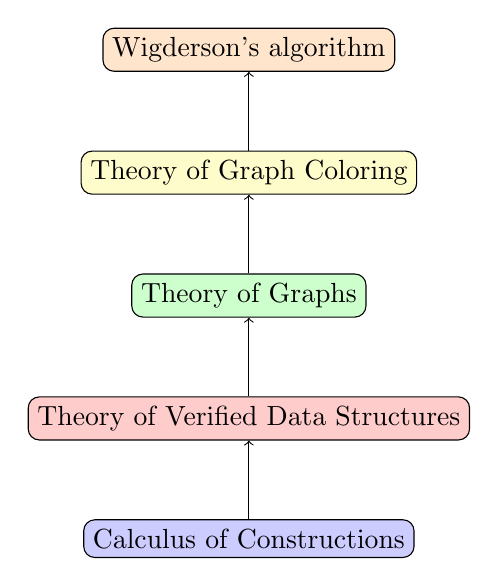
\begin{tikzpicture}

\node[rectangle, draw, fill=blue!20, text centered, rounded corners] (coc) {Calculus of Constructions};
\node[rectangle, draw, fill=red!20, text centered, rounded corners, above=of coc] (verif) {Theory of Verified Data Structures};
\node[rectangle, draw, fill=green!20, text centered, rounded corners, above=of verif] (graphs) {Theory of Graphs};
\node[rectangle, draw, fill=yellow!20, text centered, rounded corners, above=of graphs] (coloring) {Theory of Graph Coloring};
\node[rectangle, draw, fill=orange!20, text centered, rounded corners, above=of coloring] (algorithms) {Wigderson's algorithm};

\path[->] (coc) edge (verif);
\path[->] (verif) edge (graphs);
\path[->] (graphs) edge (coloring);
\path[->] (coloring) edge (algorithms);
\end{tikzpicture}
\end {figure}
\end{frame}

\begin{frame}
\frametitle{Coq Proof Assistant}
\begin{itemize}
\item Interactive theorem prover based on the Calculus of Inductive Constructions
\item Supports both dependent types and inductive types
\item Provides a rich environment for formalization and verification of mathematical proofs
\item Used in various domains, including mathematics, computer science, and software verification
\end{itemize}
\end{frame}

\begin{frame}
\frametitle{Building Graph Theory in Coq}
\begin{itemize}
\item We develop graph theory in Coq from scratch
\item Based on the definition of graphs in \cite{sf}
\item Vertices represented as positive integers
\item Adjacency set representation (a graph is a map from vertices to
  their adjacency set)
\item Conscious design choices: computable, efficient, finite
\end{itemize}
\end{frame}

\subsection{Preliminary Definitions in Coq}
\begin{frame}[fragile]
\frametitle{Preliminary Definitions in Coq}
\begin{minted}[fontsize=\footnotesize]{coq}
Module E := PositiveOrderedTypeBits.
Module S <: FSetInterface.S := PositiveSet.
Module M <: FMapInterface.S := PositiveMap.

Definition node := E.t.
Definition nodeset := S.t.
Definition nodemap: Type -> Type := M.t.
Definition graph := nodemap nodeset.

Definition adj (g: graph) (i: node) : nodeset :=
  match M.find i g with Some a => a | None => S.empty end.

Definition undirected (g: graph) :=
   forall i j, S.In j (adj g i) -> S.In i (adj g j).

Definition no_selfloop (g: graph) := forall i, ~ S.In i (adj g i).

Definition nodes (g: graph) := Mdomain g.
\end{minted}
\end{frame}

\section{Related work}
% talk about certigraph
\begin{frame}
\frametitle{Related work}
\begin{itemize}
\item Review of various formalization approaches
\item Motivations, theoretical design choices, and robustness of conclusions
\end{itemize}
\end{frame}

\section{Conclusion}
\begin{frame}
\frametitle{Conclusion}
\begin{itemize}
\item Progress towards formalization of Wigderson's graph coloring algorithm
\item Development of a reusable theory of graph coloring
\item Future research opportunities and avenues
\end{itemize}
\end{frame}

\begin{frame}
\frametitle{Acknowledgements}
\begin{itemize}
\item Thanks to advisor and mentor, Dr. Steven Tschantz, for invaluable guidance and support
\item The work leading up to the thesis and the thesis itself would not have been possible without countless extended discussions
\end{itemize}
\end{frame}

\begin{frame}
\frametitle{Questions?}
\centering
\Huge{Thank You!}
\end{frame}

\begin{frame}
\frametitle{References}
\printbibliography
\end{frame}
\end{document}
